\documentclass[man]{apa6}
\usepackage{lmodern}
\usepackage{amssymb,amsmath}
\usepackage{ifxetex,ifluatex}
\usepackage{fixltx2e} % provides \textsubscript
\ifnum 0\ifxetex 1\fi\ifluatex 1\fi=0 % if pdftex
  \usepackage[T1]{fontenc}
  \usepackage[utf8]{inputenc}
\else % if luatex or xelatex
  \ifxetex
    \usepackage{mathspec}
  \else
    \usepackage{fontspec}
  \fi
  \defaultfontfeatures{Ligatures=TeX,Scale=MatchLowercase}
\fi
% use upquote if available, for straight quotes in verbatim environments
\IfFileExists{upquote.sty}{\usepackage{upquote}}{}
% use microtype if available
\IfFileExists{microtype.sty}{%
\usepackage{microtype}
\UseMicrotypeSet[protrusion]{basicmath} % disable protrusion for tt fonts
}{}
\usepackage{hyperref}
\hypersetup{unicode=true,
            pdftitle={Maternal Emotion Dysregulation and its Association with Child Internalizing and Externalizing Behaviors and Heart Rate Variability},
            pdfauthor={Jackie O'Brien, Jenn Lewis, \& Yoel Everett},
            pdfkeywords={emotion regulation, parenting, child outcomes},
            pdfborder={0 0 0},
            breaklinks=true}
\urlstyle{same}  % don't use monospace font for urls
\usepackage{graphicx,grffile}
\makeatletter
\def\maxwidth{\ifdim\Gin@nat@width>\linewidth\linewidth\else\Gin@nat@width\fi}
\def\maxheight{\ifdim\Gin@nat@height>\textheight\textheight\else\Gin@nat@height\fi}
\makeatother
% Scale images if necessary, so that they will not overflow the page
% margins by default, and it is still possible to overwrite the defaults
% using explicit options in \includegraphics[width, height, ...]{}
\setkeys{Gin}{width=\maxwidth,height=\maxheight,keepaspectratio}
\IfFileExists{parskip.sty}{%
\usepackage{parskip}
}{% else
\setlength{\parindent}{0pt}
\setlength{\parskip}{6pt plus 2pt minus 1pt}
}
\setlength{\emergencystretch}{3em}  % prevent overfull lines
\providecommand{\tightlist}{%
  \setlength{\itemsep}{0pt}\setlength{\parskip}{0pt}}
\setcounter{secnumdepth}{0}
% Redefines (sub)paragraphs to behave more like sections
\ifx\paragraph\undefined\else
\let\oldparagraph\paragraph
\renewcommand{\paragraph}[1]{\oldparagraph{#1}\mbox{}}
\fi
\ifx\subparagraph\undefined\else
\let\oldsubparagraph\subparagraph
\renewcommand{\subparagraph}[1]{\oldsubparagraph{#1}\mbox{}}
\fi

%%% Use protect on footnotes to avoid problems with footnotes in titles
\let\rmarkdownfootnote\footnote%
\def\footnote{\protect\rmarkdownfootnote}


  \title{Maternal Emotion Dysregulation and its Association with Child
Internalizing and Externalizing Behaviors and Heart Rate Variability}
    \author{Jackie O'Brien\textsuperscript{1}, Jenn Lewis\textsuperscript{1}, \&
Yoel Everett\textsuperscript{1}}
    \date{}
  
\shorttitle{Maternal Emotion Dysregulation and Child Outcomes}
\affiliation{
\vspace{0.5cm}
\textsuperscript{1} University of Oregon}
\keywords{emotion regulation, parenting, child outcomes\newline\indent Word count: X}
\usepackage{csquotes}
\usepackage{upgreek}
\captionsetup{font=singlespacing,justification=justified}

\usepackage{longtable}
\usepackage{lscape}
\usepackage{multirow}
\usepackage{tabularx}
\usepackage[flushleft]{threeparttable}
\usepackage{threeparttablex}

\newenvironment{lltable}{\begin{landscape}\begin{center}\begin{ThreePartTable}}{\end{ThreePartTable}\end{center}\end{landscape}}

\makeatletter
\newcommand\LastLTentrywidth{1em}
\newlength\longtablewidth
\setlength{\longtablewidth}{1in}
\newcommand{\getlongtablewidth}{\begingroup \ifcsname LT@\roman{LT@tables}\endcsname \global\longtablewidth=0pt \renewcommand{\LT@entry}[2]{\global\advance\longtablewidth by ##2\relax\gdef\LastLTentrywidth{##2}}\@nameuse{LT@\roman{LT@tables}} \fi \endgroup}


\DeclareDelayedFloatFlavor{ThreePartTable}{table}
\DeclareDelayedFloatFlavor{lltable}{table}
\DeclareDelayedFloatFlavor*{longtable}{table}
\makeatletter
\renewcommand{\efloat@iwrite}[1]{\immediate\expandafter\protected@write\csname efloat@post#1\endcsname{}}
\makeatother
\usepackage{lineno}

\linenumbers

\authornote{

Correspondence concerning this article should be addressed to Jackie
O'Brien, Postal address. E-mail:
\href{mailto:my@email.com}{\nolinkurl{my@email.com}}}

\abstract{
Maternal emotion dysregulation, a transdiagnostic feature of
psychopathology, may be a potential risk factor for the emergence of
psychopathology in children. However, there is less known about child
characteristics that might serve as protective factors against this
risk. One such characteristic is heart rate variability (HRV)
reactivity, where greater decreases in HRV from baseline to a stressor
task indicate increased emotion regulation. This study examined whether
increased child HRV reactivity served as a protective factor mitigating
the transmission of psychopathology from emotionally dysregulated
mothers to behavior problems in preschool age children.

Mother-preschooler dyads (N=66) were oversampled for maternal emotion
dysregulation, measured using maternal self-report on the Difficulties
in Emotion Regulation Scale. Mothers reported on child internalizing and
externalizing behaviors using the Child Behavioral Checklist. Child
baseline HRV was collected, where the child sat quietly for 2 minutes
while a book was read to them. Child HRV was also measured during a
stressor task, where dyads had 7 minutes to build a complex Lego figure.
HRV reactivity was calculated by subtracting child baseline HRV from
child HRV during the stressor task.

Two hierarchical regression models were conducted, entering maternal
emotion dysregulation, child HRV reactivity, and the interaction term of
these variables predicting either child internalizing or child
externalizing problems (see Table 1). Across these two models, maternal
emotion dysregulation, but not child HRV reactivity, significantly
predicted child's internalizing and externalizing behaviors. Maternal
emotion dysregulation significantly interacted with child HRV reactivity
to predict child internalizing behaviors, such that maternal emotion
dysregulation had a greater impact on child internalizing behaviors if
the child exhibited a greater decrease in HRV from baseline to the
stressor task (i.e.~exhibited increased self-regulation). There was no
significant interaction predicting child externalizing behaviors.

These findings suggest that maternal emotion dysregulation more strongly
predicts child behavior problems in physiologically regulated children.
Interventions that target maternal emotion dysregulation may therefore
improve child behavior outcomes even in physiologically regulated
children.


}

\begin{document}
\maketitle

\section{Introduction}\label{introduction}

Emotion dysregulation, a transdiagnostic feature of psychopathology, has
been shown to be a significant mediator of mental health symptoms and
symptom severity in adults. A parent's own mental health has been known
to predict child mental health symptoms and behavioral problems. These
two facts together, therefore, may mean a parent's emotion regulation,
particularly emotion regulation difficulties, may be an important risk
factor for the emergence of psychopathology in children. Investigating
the role of parental emotion regulation on childhood health and mental
health problems is therfore an important clinical question in need of
further investigation.

While risk factors are one important area to investigate in the
prevention of child mental health symptoms, it is also important to
examine protective factors that may help make a child more resilient to
developing these symptoms later on. However, there is less known about
child characteristics that might serve as protective factors against
risk. One such characteristic that has been identified in the literature
is heart rate variability (HRV) reactivity, where greater decreases in
HRV from baseline to a stressor task indicate increased emotion
regulation.

This study examined whether increased child HRV reactivity served as a
protective factor mitigating the transmission of psychopathology from
emotionally dysregulated mothers to behavior problems in preschool age
children. The aims of this research is to investigate the relationship
between maternal emotion dysregulation and child behaviors in a sample
of women with BPD symptoms and there preschool aged children. A second
aim is to examine the effects of maternal emotion dysregulation on child
HRV reactivity. The final aim is to examine the interaction of maternal
emotion dysregulation and child reactivity on child behaviors.

\section{Methods}\label{methods}

\subsection{Participants}\label{participants}

Sixty-eight mothers and their preschool aged children (M = 48, SD = 7.6
months, 46\% girls) were recruited from various sources including a
developmental database maintained by the university psychology
department, craigslist, and community mental health centers. Mothers
were recruited based on the presence or absence of borderline
personality disorder (BPD) symptoms, a disorder marked by extreme
emotion dysregulation, as measured by the McLean screener (Zanarini et
al., 2003). Mothers with elevated BPD symptoms were oversampled in order
to ensure a range of emotion regulatory capabilities.

\subsection{Procedure}\label{procedure}

Families participated in a 2.5-hour assessment in offices on a
university campus. Prior to participation, both mother consent and child
assent were obtained, per Institutional Review Board approval. While
mothers completed questionnaires, children completed assessments in an
adjacent room, although child assessment data is not presented here.
Mother and children were then reunited for parent-child interaction
tasks in which baseline and stressor task HRV was collected on both
mothers and children. Only child HRV data is presented here.

\subsection{Materials}\label{materials}

\textbf{Maternal emotion dysregulation.} Maternal emotion dysregulation
was measured using the Difficulties in Emotion Regulation Scale (DERS;
Gratz \& Roemer, 2004). The DERS is a 36-item self-report questionnaire
designed to assess multiple facets of emotional dysregulation, with
scores ranging from 36-180 (\emph{M}=70.10, \emph{SD}=22.33). Higher
scores suggest greater emotion dysregulation.

\textbf{Heart rate variability.} Child baseline HRV was collected, where
the child sat quietly for 2 minutes while a book was read to them. Child
HRV was also measured during a stressor task, where dyads had 7 minutes
to build a complex Lego figure. HRV reactivity was calculated by
subtracting child baseline HRV from child HRV during the stressor task
(\emph{M}=NA, \emph{SD}=NA)..

\textbf{Child behavior problems.} Child behavior problems were assessed
using maternal report on the Child Behavior Checklist (CBCL) for both
internalizing (i.e., anxious, depressive, and overcontrolled) and
externalizing (i.e., aggressive, hyperactive, noncompliant, and
undercontrolled) behaviors. Mean scores are presented in Table 2.

\subsection{Data analysis}\label{data-analysis}

We used R (Version 3.5.1; R Core Team, 2018) and the R-packages
\emph{bindrcpp} (Version 0.2.2; Müller, 2018), \emph{dplyr} (Version
0.7.6; Wickham, François, Henry, \& Müller, 2018), \emph{forcats}
(Version 0.3.0; Wickham, 2018a), \emph{ggplot2} (Version 3.0.0; Wickham,
2016), \emph{here} (Version 0.1; Müller, 2017), \emph{jtools} (Version
1.1.1; Long, 2018), \emph{kableExtra} (Version 0.9.0; Zhu, 2018),
\emph{knitr} (Version 1.20; Xie, 2015), \emph{papaja} (Version
0.1.0.9842; Aust \& Barth, 2018), \emph{purrr} (Version 0.2.5; Henry \&
Wickham, 2018), \emph{readr} (Version 1.1.1; Wickham, Hester, \&
Francois, 2017), \emph{rio} (Version 0.5.10; C.-h. Chan, Chan, Leeper,
\& Becker, 2018), \emph{stringr} (Version 1.3.1; Wickham, 2018b),
\emph{tibble} (Version 1.4.2; Müller \& Wickham, 2018), \emph{tidyr}
(Version 0.8.1; Wickham \& Henry, 2018), and \emph{tidyverse} (Version
1.2.1; Wickham, 2017) for all our analyses.

\section{Results}\label{results}

Means and standard deviations for variables are presented in Table 1.
and Table 2.

Two hierarchical regression models were conducted, entering maternal
emotion dysregulation, child HRV reactivity, and the interaction term of
these variables predicting either child internalizing or child
externalizing problems (see Table 2.). Across these two models, maternal
emotion dysregulation, but not child HRV reactivity, significantly
predicted child's internalizing and externalizing behaviors. Maternal
emotion dysregulation significantly interacted with child HRV reactivity
to predict child internalizing behaviors, such that maternal emotion
dysregulation had a greater impact on child internalizing behaviors if
the child exhibited a greater decrease in HRV from baseline to the
stressor task (i.e.~exhibited increased self-regulation). There was no
significant interaction predicting child externalizing behaviors.

\begin{table}[tbp]
\begin{center}
\begin{threeparttable}
\caption{\label{tab:descriptives ders and reactivity}Means and SDs for Maternal Emotion Dysregulation (DERS) and Child Reactivity}
\begin{tabular}{llll}
\toprule
DERS\_mean & \multicolumn{1}{c}{DERS\_SD} & \multicolumn{1}{c}{Reactivity\_mean} & \multicolumn{1}{c}{Reactivity\_SD}\\
\midrule
70.10 & 22.33 & -1.10 & 0.65\\
\bottomrule
\end{tabular}
\end{threeparttable}
\end{center}
\end{table}

\begin{table}[tbp]
\begin{center}
\begin{threeparttable}
\caption{\label{tab:descriptives cbcl}Means and SDs for Child Internalizing and Externalizing Behavior}
\begin{tabular}{lll}
\toprule
cbcl\_subtype & \multicolumn{1}{c}{cbcl\_mean} & \multicolumn{1}{c}{cbcl\_SD}\\
\midrule
ext & 16.28 & 9.49\\
int & 11.17 & 7.54\\
\bottomrule
\end{tabular}
\end{threeparttable}
\end{center}
\end{table}

\begin{table}[tbp]
\begin{center}
\begin{threeparttable}
\caption{\label{tab:linear regression internalizing}Results of Linear Regression Predicting Child Internalizing Behavior}
\begin{tabular}{lllll}
\toprule
Predictor & \multicolumn{1}{c}{$b$} & \multicolumn{1}{c}{95\% CI} & \multicolumn{1}{c}{$t(45)$} & \multicolumn{1}{c}{$p$}\\
\midrule
Intercept & 11.00 & $[9.04$, $12.97]$ & 11.27 & < .001\\
Ders c & 0.17 & $[0.08$, $0.25]$ & 3.98 & < .001\\
Reactivity c & -1.19 & $[-4.30$, $1.91]$ & -0.77 & .443\\
Ders c $\times$ Reactivity c & -0.18 & $[-0.34$, $-0.02]$ & -2.27 & .028\\
\bottomrule
\end{tabular}
\end{threeparttable}
\end{center}
\end{table}

\begin{table}[tbp]
\begin{center}
\begin{threeparttable}
\caption{\label{tab:linear regression externalizing}Results of Linear Regression Predicting Child Externalizing Behavior}
\begin{tabular}{lllll}
\toprule
Predictor & \multicolumn{1}{c}{$b$} & \multicolumn{1}{c}{95\% CI} & \multicolumn{1}{c}{$t(45)$} & \multicolumn{1}{c}{$p$}\\
\midrule
Intercept & 16.02 & $[13.34$, $18.69]$ & 12.06 & < .001\\
Ders c & 0.16 & $[0.05$, $0.27]$ & 2.84 & .007\\
Reactivity c & 1.72 & $[-2.50$, $5.94]$ & 0.82 & .415\\
Ders c $\times$ Reactivity c & -0.03 & $[-0.25$, $0.19]$ & -0.30 & .764\\
\bottomrule
\end{tabular}
\end{threeparttable}
\end{center}
\end{table}

\begin{figure}
\centering
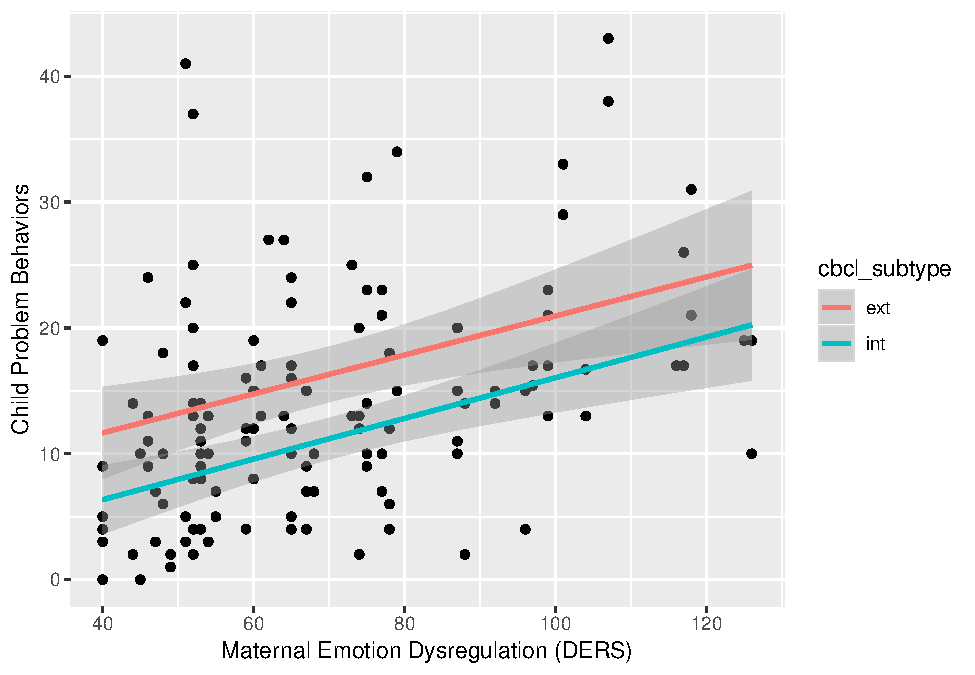
\includegraphics{DataPrepScript_apa_style_files/figure-latex/plot1-1.pdf}
\caption{\label{fig:plot1}Maternal Emotion Dysregulation and Child
Behaviors}
\end{figure}

\begin{figure}
\centering
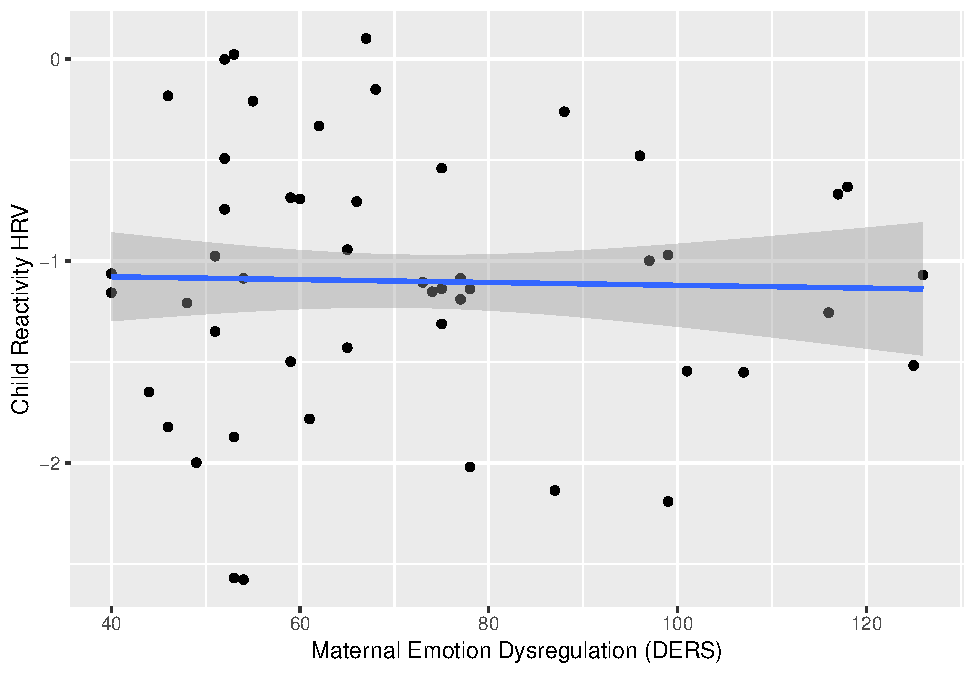
\includegraphics{DataPrepScript_apa_style_files/figure-latex/plot2-1.pdf}
\caption{\label{fig:plot2}Maternal Emotion Dysregulation and Child HRV
Reactivity}
\end{figure}

\begin{figure}
\centering
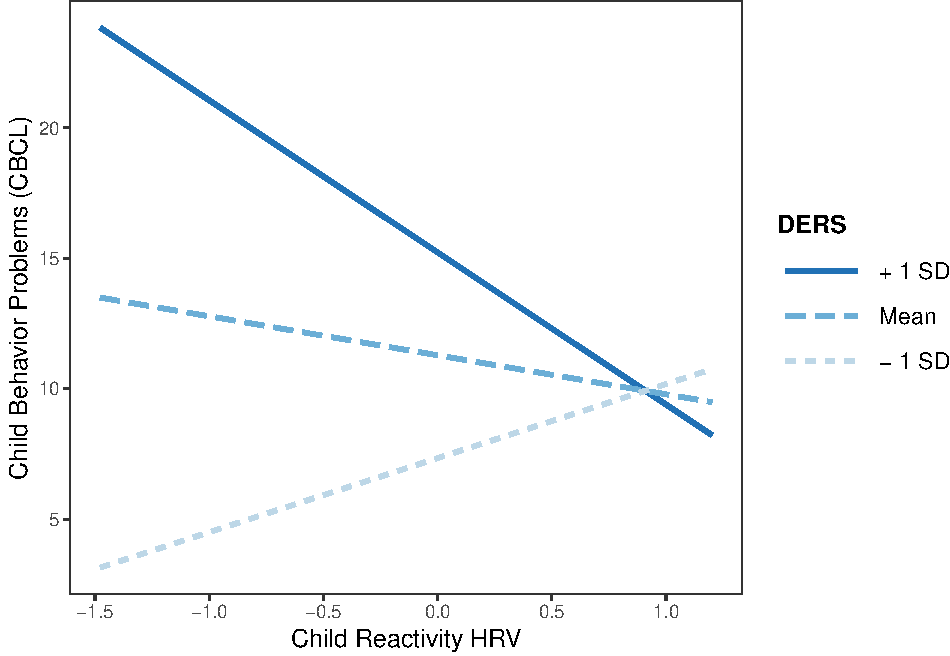
\includegraphics{DataPrepScript_apa_style_files/figure-latex/plot3-1.pdf}
\caption{\label{fig:plot3}Child Reactivity Predicting Child Behavior
Problems at Three Different Levels of Maternal Emotion Dysregulation}
\end{figure}

\section{Discussion}\label{discussion}

These findings suggest that maternal emotion dysregulation more strongly
predicts child behavior problems in physiologically regulated children.
Interventions that target maternal emotion dysregulation may therefore
improve child behavior outcomes even in physiologically regulated
children.

\newpage

\section{References}\label{references}

\begingroup
\setlength{\parindent}{-0.5in} \setlength{\leftskip}{0.5in}

\hypertarget{refs}{}
\hypertarget{ref-R-papaja}{}
Aust, F., \& Barth, M. (2018). \emph{papaja: Create APA manuscripts with
R Markdown}. Retrieved from \url{https://github.com/crsh/papaja}

\hypertarget{ref-R-rio}{}
Chan, C.-h., Chan, G. C., Leeper, T. J., \& Becker, J. (2018).
\emph{Rio: A swiss-army knife for data file i/o}.

\hypertarget{ref-R-purrr}{}
Henry, L., \& Wickham, H. (2018). \emph{Purrr: Functional programming
tools}. Retrieved from \url{https://CRAN.R-project.org/package=purrr}

\hypertarget{ref-R-jtools}{}
Long, J. A. (2018). \emph{Jtools: Analysis and presentation of social
scientific data}. Retrieved from
\url{https://cran.r-project.org/package=jtools}

\hypertarget{ref-R-here}{}
Müller, K. (2017). \emph{Here: A simpler way to find your files}.
Retrieved from \url{https://CRAN.R-project.org/package=here}

\hypertarget{ref-R-bindrcpp}{}
Müller, K. (2018). \emph{Bindrcpp: An 'rcpp' interface to active
bindings}. Retrieved from
\url{https://CRAN.R-project.org/package=bindrcpp}

\hypertarget{ref-R-tibble}{}
Müller, K., \& Wickham, H. (2018). \emph{Tibble: Simple data frames}.
Retrieved from \url{https://CRAN.R-project.org/package=tibble}

\hypertarget{ref-R-base}{}
R Core Team. (2018). \emph{R: A language and environment for statistical
computing}. Vienna, Austria: R Foundation for Statistical Computing.
Retrieved from \url{https://www.R-project.org/}

\hypertarget{ref-R-ggplot2}{}
Wickham, H. (2016). \emph{Ggplot2: Elegant graphics for data analysis}.
Springer-Verlag New York. Retrieved from \url{http://ggplot2.org}

\hypertarget{ref-R-tidyverse}{}
Wickham, H. (2017). \emph{Tidyverse: Easily install and load the
'tidyverse'}. Retrieved from
\url{https://CRAN.R-project.org/package=tidyverse}

\hypertarget{ref-R-forcats}{}
Wickham, H. (2018a). \emph{Forcats: Tools for working with categorical
variables (factors)}. Retrieved from
\url{https://CRAN.R-project.org/package=forcats}

\hypertarget{ref-R-stringr}{}
Wickham, H. (2018b). \emph{Stringr: Simple, consistent wrappers for
common string operations}. Retrieved from
\url{https://CRAN.R-project.org/package=stringr}

\hypertarget{ref-R-tidyr}{}
Wickham, H., \& Henry, L. (2018). \emph{Tidyr: Easily tidy data with
'spread()' and 'gather()' functions}. Retrieved from
\url{https://CRAN.R-project.org/package=tidyr}

\hypertarget{ref-R-dplyr}{}
Wickham, H., François, R., Henry, L., \& Müller, K. (2018). \emph{Dplyr:
A grammar of data manipulation}. Retrieved from
\url{https://CRAN.R-project.org/package=dplyr}

\hypertarget{ref-R-readr}{}
Wickham, H., Hester, J., \& Francois, R. (2017). \emph{Readr: Read
rectangular text data}. Retrieved from
\url{https://CRAN.R-project.org/package=readr}

\hypertarget{ref-R-knitr}{}
Xie, Y. (2015). \emph{Dynamic documents with R and knitr} (2nd ed.).
Boca Raton, Florida: Chapman; Hall/CRC. Retrieved from
\url{https://yihui.name/knitr/}

\hypertarget{ref-R-kableExtra}{}
Zhu, H. (2018). \emph{KableExtra: Construct complex table with 'kable'
and pipe syntax}. Retrieved from
\url{https://CRAN.R-project.org/package=kableExtra}

\endgroup


\end{document}
